\documentclass[aspectratio=169,11pt]{beamer}
\usepackage[T1]{fontenc}
\usepackage{lmodern,amsmath,amssymb,mathtools,bm,booktabs,array,graphicx,tikz}
\usetikzlibrary{arrows.meta,positioning,calc,decorations.pathreplacing,patterns}
\definecolor{ink}{HTML}{17344D}\definecolor{accent}{HTML}{087E8B}\definecolor{pale}{HTML}{EDF5F5}\definecolor{gold}{HTML}{AD6B19}
\providecommand{\dd}{\,\mathrm{d}}\providecommand{\R}{\mathbb{R}}
\providecommand{\E}{\mathbb{E}}\providecommand{\Var}{\operatorname{Var}}
\providecommand{\Cov}{\operatorname{Cov}}\providecommand{\diag}{\operatorname{diag}}
\providecommand{\norm}[1]{\left\lVert#1\right\rVert}
\providecommand{\abs}[1]{\left|#1\right|}
\usefonttheme{professionalfonts}
\setbeamercolor{normal text}{fg=black,bg=white}
\setbeamercolor{frametitle}{fg=ink,bg=white}
\setbeamercolor{title}{fg=ink}\setbeamercolor{structure}{fg=accent}
\setbeamercolor{block title}{fg=ink,bg=pale}\setbeamercolor{block body}{fg=black,bg=pale!40}
\setbeamercolor{alerted text}{fg=accent}
\setbeamerfont{frametitle}{size=\Large,series=\bfseries}
\setbeamerfont{title}{size=\LARGE,series=\bfseries}
\setbeamertemplate{navigation symbols}{}
\setbeamersize{text margin left=.7cm,text margin right=.7cm}
\setbeamertemplate{frametitle}{\vspace{.18cm}\insertframetitle\par\vspace{.1cm}{\color{accent}\hrule height .6pt}\vspace{.12cm}}
\newcommand{\notestarget}{notes.pdf}\newcommand{\noteslabel}{Notes}
\setbeamertemplate{footline}{\hspace{.7cm}\color{ink}\scriptsize Computational Cardiology\quad\href{\notestarget}{\noteslabel}\hfill\insertframenumber\,/\,\inserttotalframenumber\hspace{.7cm}\vspace{.18cm}}
\setbeamercovered{invisible}
\hypersetup{pdfauthor={Zan Ahmad},pdftitle={Cardiac phase and pressure feedback in a pulsatile circulation},pdfpagemode=UseNone}
\begin{document}
\begin{frame}[plain]\vfill
{\small\color{accent} Computational Cardiology \quad Lecture 4}\par\medskip
{\raggedright\hyphenpenalty=10000\exhyphenpenalty=10000\LARGE\bfseries\color{ink} Cardiac phase and pressure feedback in a pulsatile circulation}\par\bigskip
Zan Ahmad\par\smallskip
{\small Fall 2024}\par\vfill\end{frame}
\renewcommand{\notestarget}{notes.pdf\#note-the-circulation-boundary-and-constitutive-laws}
\begin{frame}[label=slide-storage-and-boundary-conditions-figure]{The two-pump circulation}
\centering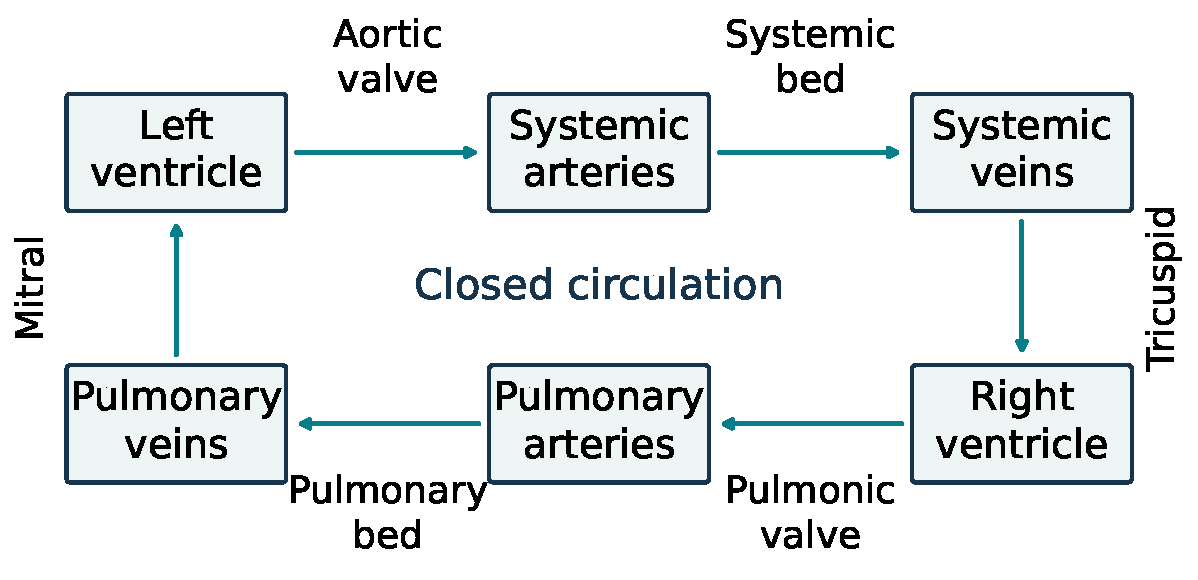
\includegraphics[width=.98\linewidth,height=.69\textheight,keepaspectratio]{presentation-figures/circuit-panel-1.pdf}\end{frame}
\renewcommand{\notestarget}{notes.pdf\#note-the-circulation-boundary-and-constitutive-laws}
\begin{frame}[t,fragile,label=slide-storage-and-boundary-conditions]{Storage and boundary conditions}
\[V_i=V_{d,i}+C_i(\phi)P_i.\]\pause{} The six-region companion is closed. The source feedback paper uses a ventricle and arterial storage with prescribed reservoirs.
\end{frame}
\renewcommand{\notestarget}{notes.pdf\#note-the-circulation-boundary-and-constitutive-laws}
\begin{frame}[t,fragile,label=slide-a-valve-conducts-only-forward]{A valve conducts only forward}
\[q_{ij}=\frac{[P_i-P_j]_+}{R_{ij}},\qquad [z]_+=\max(z,0).\]\pause{} Vascular beds remain open resistors with signed flow.
\end{frame}
\renewcommand{\notestarget}{notes.pdf\#note-the-circulation-boundary-and-constitutive-laws}
\begin{frame}[t,fragile,label=slide-contraction-changes-the-pressure-law]{Contraction changes the pressure law}
\[\frac{\mathrm d}{\mathrm dt}(CP)=C\dot P+\dot CP=q_{\rm in}-q_{\rm out}.\]\pause{} At fixed volume, decreasing $C$ raises $P$.
\end{frame}
\renewcommand{\notestarget}{notes.pdf\#note-conservative-implicit-hydraulics}
\begin{frame}[t,fragile,label=slide-the-implicit-hydraulic-step]{The implicit hydraulic step}
\[(D_C^{n+1}+hL_{\rm active})P^{n+1}=D_C^nP^n.\]\pause{} Valve labels must agree with the resulting new-pressure differences.
\end{frame}
\renewcommand{\notestarget}{notes.pdf\#note-filtered-pressure-and-bounded-proportional-control}
\begin{frame}[t,fragile,label=slide-filter-the-arterial-pressure]{Filter the arterial pressure}
\[\tau\frac{\mathrm d\bar P}{\mathrm dt}=P_{sa}-\bar P.\]\pause{} The time constant separates the controller input from the rapid pressure pulse.
\end{frame}
\renewcommand{\notestarget}{notes.pdf\#note-filtered-pressure-and-bounded-proportional-control}
\begin{frame}[t,fragile,label=slide-the-filter-update]{The filter update}
\[\bar P^{n+1}=\bar P^n+\frac h\tau(P_{sa}^n-\bar P^n).\]\pause{} For $0\le h/\tau\le1$, the update lies between the two old pressures.
\end{frame}
\renewcommand{\notestarget}{notes.pdf\#note-filtered-pressure-and-bounded-proportional-control}
\begin{frame}[t,fragile,label=slide-bounded-proportional-rate-control]{Bounded proportional rate control}
\[F=\operatorname{clip}\!\left(F_0\left[1+g\frac{P_* -\bar P}{P_*}\right],F_{\min},F_{\max}\right).\]\pause{} Low filtered pressure increases the requested heart rate.
\end{frame}
\renewcommand{\notestarget}{notes.pdf\#note-the-accumulated-cardiac-clock}
\begin{frame}[t,fragile,label=slide-a-continuously-varying-clock]{A continuously varying clock}
\[\dot\phi=F(t),\qquad \phi(t)=\phi(0)+\int_0^tF(s)\,\mathrm ds.\]\pause{} The compliance sequence is unchanged; the speed through it varies.
\end{frame}
\renewcommand{\notestarget}{notes.pdf\#note-the-accumulated-cardiac-clock}
\begin{frame}[t,fragile,label=slide-why-phase-is-not-current-rate-times-time]{Why phase is not current rate times time}
\[\frac{\mathrm d}{\mathrm dt}[tF(t)]=F(t)+t\dot F(t).\]\pause{} If $F(t)=F_0+at$, correct phase is $F_0t+at^2/2$, not $F_0t+at^2$.
\end{frame}
\renewcommand{\notestarget}{notes.pdf\#note-the-accumulated-cardiac-clock}
\begin{frame}[t,fragile,label=slide-one-phase-for-both-ventricles]{One phase for both ventricles}
\[\phi^{n+1}=\phi^n+\frac{h_s}{60}F^{n+1}.\]\pause{} Both ventricular compliance laws use this accumulated phase. Seconds and minutes remain distinct.
\end{frame}
\renewcommand{\notestarget}{notes.pdf\#note-a-prescribed-resistance-disturbance}
\begin{frame}[label=slide-a-resistance-disturbance-panel-1]{Arterial pressure under feedback}
\centering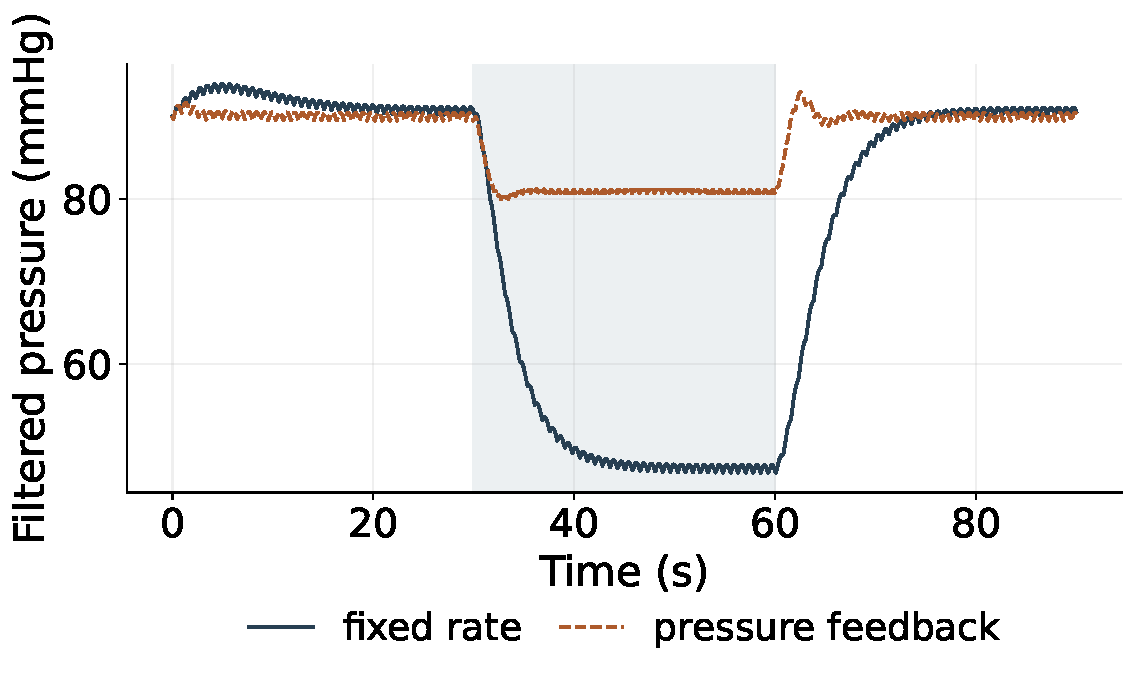
\includegraphics[width=.98\linewidth,height=.69\textheight,keepaspectratio]{presentation-figures/feedback-response-panel-1.pdf}\end{frame}
\renewcommand{\notestarget}{notes.pdf\#note-a-prescribed-resistance-disturbance}
\begin{frame}[label=slide-a-resistance-disturbance-panel-2]{Systemic flow under feedback}
\centering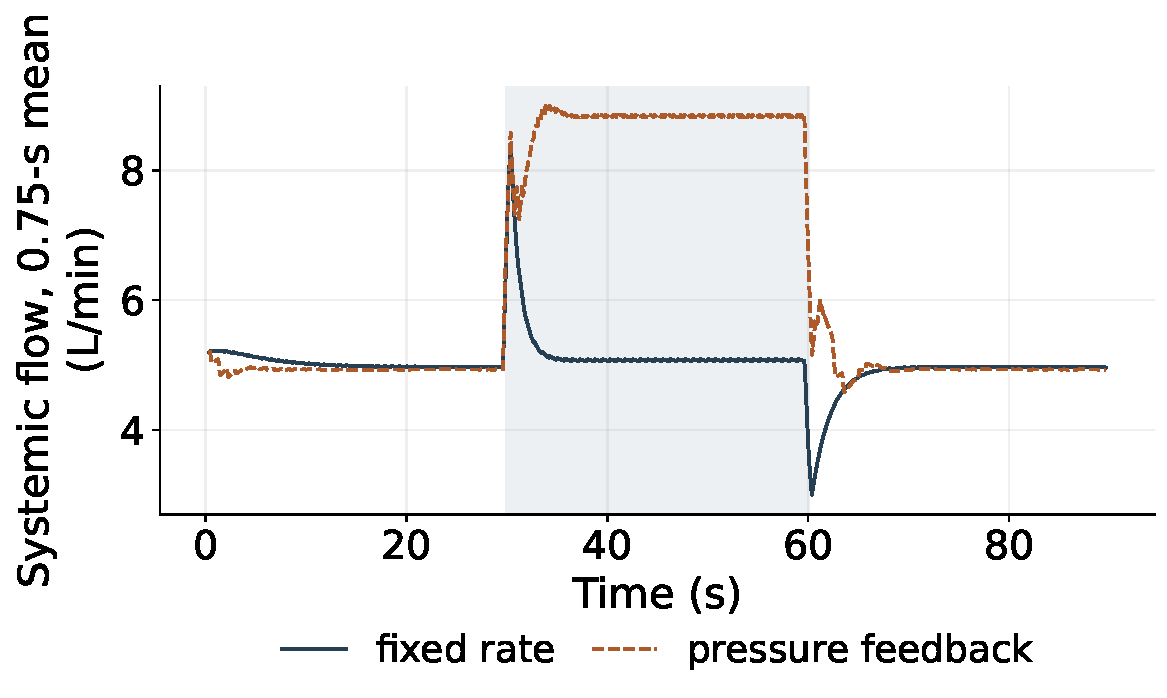
\includegraphics[width=.98\linewidth,height=.69\textheight,keepaspectratio]{presentation-figures/feedback-response-panel-2.pdf}\end{frame}
\renewcommand{\notestarget}{notes.pdf\#note-a-prescribed-resistance-disturbance}
\begin{frame}[label=slide-a-resistance-disturbance-panel-3]{Heart rate under feedback}
\centering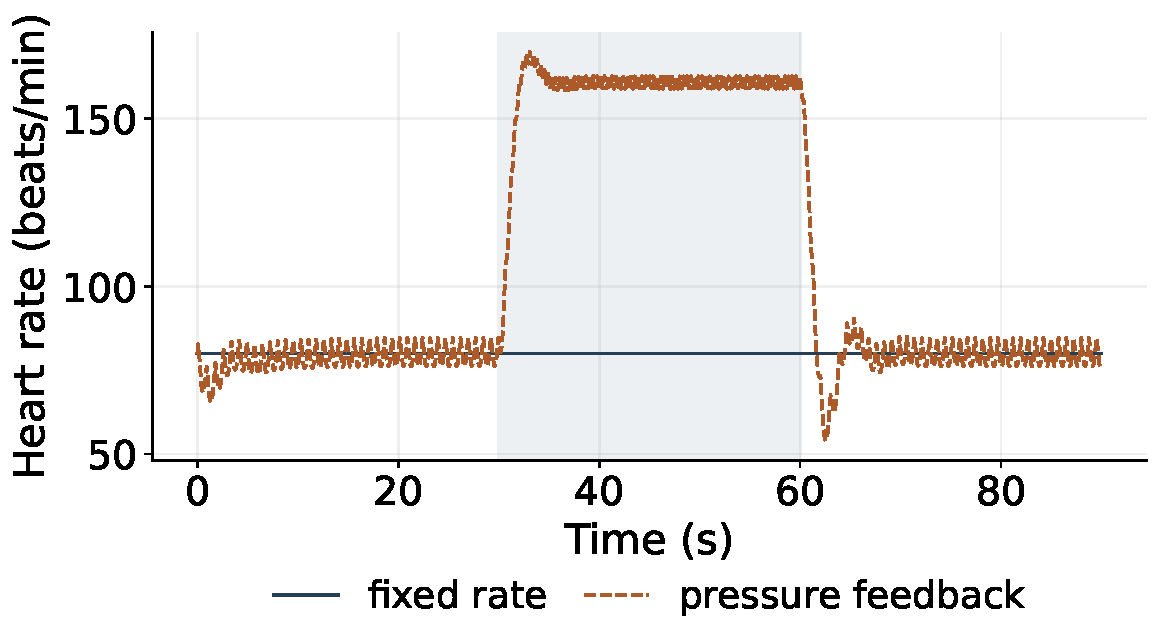
\includegraphics[width=.98\linewidth,height=.69\textheight,keepaspectratio]{presentation-figures/feedback-response-panel-3.pdf}\end{frame}
\renewcommand{\notestarget}{notes.pdf\#note-a-prescribed-resistance-disturbance}
\begin{frame}[t,fragile,label=slide-a-resistance-disturbance]{A resistance disturbance}
\[R_s:17.86\longrightarrow8.93\longrightarrow17.86\quad\mathrm{mmHg\,min/L}.\]\pause{} The reductions begin at $30$ s and end at $60$ s in the supplied experiment.
\end{frame}
\renewcommand{\notestarget}{notes.pdf\#note-a-prescribed-resistance-disturbance}
\begin{frame}[t,fragile,label=slide-the-required-mean-flow-change]{The required mean-flow change}
\[\overline Q_s\simeq\frac{\Delta\overline P_s}{R_s}.\]\pause{} At a fixed pressure drop, halving resistance requires twice the flow. The coupled pressures need not remain fixed.
\end{frame}
\renewcommand{\notestarget}{notes.pdf\#note-equilibrium-offsets-and-numerical-sensitivity}
\begin{frame}[t,fragile,label=slide-the-proportional-control-offset]{The proportional-control offset}
\[\frac{P_* -\bar P}{P_*}=\frac{F_{\rm req}/F_0-1}{g}.\]\pause{} A rate above baseline requires a pressure shortfall when the target and gain are fixed and clipping is inactive.
\end{frame}
\renewcommand{\notestarget}{notes.pdf\#note-equilibrium-offsets-and-numerical-sensitivity}
\begin{frame}[t,fragile,label=slide-gain-and-delayed-response]{Gain and delayed response}
The pressure filter and blood redistribution delay the rate response.\pause{} A larger gain reduces the static offset while potentially increasing oscillatory transient behavior.
\end{frame}
\renewcommand{\notestarget}{notes.pdf\#note-equilibrium-offsets-and-numerical-sensitivity}
\begin{frame}[t,fragile,label=slide-quantities-retained-by-this-controller]{Quantities retained by this controller}
Rate control changes cycle timing. It does not independently regulate contractility, vascular tone or venous return.\pause{} A centered plotting average is not the causal pressure filter used by the controller.
\end{frame}
\end{document}
